% b2026 paper v0.1 (20260822)
% Target: arXiv cs.AR, then a journal (ACM TRETS preferred).
% TODO before submission:
%   - add the repository URL once the code is public
\documentclass[11pt,a4paper]{article}

\usepackage[T1]{fontenc}
\usepackage[utf8]{inputenc}
\usepackage{geometry}
\geometry{margin=2.5cm}
\usepackage{booktabs}
\usepackage{listings}
\usepackage{amsmath}
\usepackage{tikz}
\usetikzlibrary{positioning,arrows.meta,fit,backgrounds}
\usepackage[hidelinks]{hyperref}

\setlength{\parindent}{0pt}
\setlength{\parskip}{0.6em}
\setcounter{topnumber}{1}

\lstset{basicstyle=\ttfamily\small, frame=single, captionpos=b,
        columns=fullflexible, showstringspaces=false}

\title{B2026: A Machine With No Instruction Set\\
Reviving the Burroughs B1700 Soft Machine on a Modern FPGA}

\author{Senol Gulgonul\\
Department of Electrical and Electronics Engineering\\
OSTIM Technical University, Ankara, Turkey\\
\texttt{senol.gulgonul@ostimteknik.edu.tr}\\
\url{https://orcid.org/0000-0001-5346-4448}}

\date{\today}

\begin{document}
\maketitle

\begin{abstract}
B2026 is a soft machine for a 8640-LUT FPGA whose hardware implements
no instruction set. Memory is addressed to the bit through a field
isolation unit, an operand-length register reshapes the arithmetic unit
every cycle, and the control store is written at run time, so an
instruction set is data rather than a synthesis artifact. RV32I is one
S-language in 838 microwords, passing riscv-tests rv32ui 42 of 42 with
misaligned access free because memory is bit addressed; a byte-coded
stack machine is another in 75 microwords, and the two are exchanged
over a serial line in about a second without resynthesis. On the same
board, wrapper and workload, the design costs 2569 LUT against 236 for
Glacial, 283 for SERV and 1097 for PicoRV32, and reaches 29.7 MHz at
81.3 cycles per instruction. On every axis a fixed-ISA core optimizes
for, a definable machine loses; the comparison has no column for what
is bought. These measurements put a number on the premise of the
Burroughs B1700, to which the design owes its principles and its name.
\end{abstract}

\section{Introduction}

Procrustes, in the story Wilner opens with, stretched or cut his guests
to fit an iron bed. The complaint against von Neumann derived machines
was the same: memory cells and processor registers are rigid containers
that force data and instructions into unnatural shapes, and a small
fixed set of machine operations is a poor fit for the range of
algorithms people actually write. The Burroughs B1700 was the answer,
and its thesis was quantitative rather than aesthetic: accommodating a
definable structure from instruction to instruction costs less than the
waste incurred when one structure serves everything.

The machine that followed from this had no instruction set. Programs
were expressed in an S-language, a machine language chosen or invented
for the application area, and an interpreter written in microcode gave
the hardware the shape that language needed. Memory was addressed to
the bit; a field isolation unit extracted and inserted arbitrary bit
strings; bias registers reshaped the data path on a clock by clock
basis; and interpreters lived in ordinary memory as named files,
loadable and switchable between any two S-instructions.

Fifty-four years later the hardware assumptions have inverted. Logic is
abundant and cheap, memory on a small FPGA is scarce and precious, and
the dominant instruction set is an open standard that everyone
implements identically. That inversion makes the B1700 premise worth
re-testing rather than merely admiring, and the test is now cheap
enough to run on a twenty dollar board.

This paper reports such a test. The machine is called B2026, in homage
to the B1700 and to nothing else: it is not a Burroughs product and
implements no Burroughs instruction set. Section~\ref{sec:arch}
describes it as built for a Gowin GW1NR-9. Section
\ref{sec:rv32i} presents RV32I as its first S-language and the
verification of that interpreter. Section~\ref{sec:store} describes the
writable control store, the resident loader and the console services
that the loader exports to interpreters. Section~\ref{sec:swap} shows
two S-languages exchanged on one bitstream. Section~\ref{sec:results}
gives synthesis, timing and cycle measurements against three fixed-ISA
cores on the same board.

\section{Related work}

Microprogramming as a way of trading logic for memory dates to
Wilkes~\cite{wilkes1951}, who proposed a matrix of stored control
signals in place of a wired sequencer. The B1700~\cite{wilner1972}
extended the idea past control into the representation of data itself,
and Barton's earlier survey of ideas for computer systems
organization~\cite{barton1970} supplied several of its design
objectives.

Among contemporary FPGA cores, three are directly comparable and are
used as baselines here. SERV~\cite{serv} is a bit-serial RV32I core that reaches
its small size by processing one bit per cycle. PicoRV32~\cite{picorv32} is a
size-optimized but conventionally parallel RV32I core.
Glacial~\cite{glacial} is the closest relative: a microcoded RV32I core with an eight bit data path
that keeps microcode, scratchpad and RISC-V memory in one byte-wide
RAM, deliberately trading logic cells for RAM and slower execution.
Freeman's minimal CISC processor for FPGAs makes the same trade in the
control path, placing microprogrammed control in block RAM to reduce
slice count~\cite{freeman2004}.

The distance between this work and those cores is not microcoding, and
in Glacial's case not even the placement of microcode in memory. It is
that in all of them the microcode implements a fixed instruction set
and is frozen at synthesis. Here the hardware is committed to no
instruction set at all, the control store is rewritten at run time, and
the interpreted language is a parameter of the running system.

\section{Architecture}
\label{sec:arch}

The machine is a small single-cycle micromachine with a writable
control store, a defined-field memory interface and a bias register.
Five principles are carried over from the original.

\emph{Defined-field access.} Memory is addressed by a triple of bit
address, length and direction. A field isolation unit sits in front of
conventional 32-bit block RAM and performs extraction and
read-modify-write insertion. Addresses label positions between bits, so
that reading $L$ bits forward from address $a$ returns the same field
as reading $L$ bits backward from $a+L$, a property the original used
to make microcode read the way programmers think about bit strings.

\emph{Bias.} A current-operand-length register, CPL, reshapes the
function box every cycle. The carry out is taken from bit $\mathrm{CPL}-1$,
the zero and sign flags are computed on the masked result, and operands
are masked to CPL before use. Microcode that loads CPL from a
descriptor therefore behaves correctly whatever the operand width.

\emph{Microcode is software.} The control store is written at run time
by a microinstruction, so an interpreter is data rather than a
synthesis artifact.

\emph{Interpreted machine state lives in memory.} For RV32I the
architectural registers and the program counter are fields in
S-memory, not hardware registers, so an interpreter can be suspended
between any two interpreted instructions with no hidden state.

\emph{Readable microassembly.} One statement per microinstruction, in
the spirit of the original MIL.

The function box follows the B1700 arrangement in which the programmer
does not execute an addition but reads a sum. Two operand registers
feed a combinational box whose outputs, sum, difference, and the three
bitwise functions, are all available every cycle as read-only register
names; a move instruction selects one. Table~\ref{tab:micro} lists the
microinstruction classes.

\begin{table}[!htb]
\centering
\caption{The sixteen microinstruction classes of the vertical 16-bit
microword.}
\label{tab:micro}
\begin{tabular}{@{}lll@{}}
\toprule
Class & Mnemonic & Effect \\
\midrule
0 & MOVE & register to register, 6-bit source and destination names \\
1, 2 & LIT, LITS & build a literal in T, twelve bits at a time \\
3, 4 & READ, WRITE & defined-field access through F or SF, with counting \\
5 & EXT & extract CPL bits from X at a literal position \\
6, 7 & BR, IF & relative transfer, twelve conditions \\
8, 9 & CALL, EXIT & microsubroutine call and return, 16-deep stack \\
A & DISP & dispatch to a page indexed by the low byte of T \\
B & BIAS & load CPL from a literal or a descriptor length \\
C & CNT & count a descriptor address or length up or down \\
F & CTRL & halt, monitor, console access, control store write \\
\bottomrule
\end{tabular}
\end{table}

Figure~\ref{fig:arch} shows how these pieces fit together. Two paths in
it carry the argument of the paper. The bias path takes CPL into the
function box, where it decides how wide the operands are and where the
carry comes from, and the write path takes a datum from the machine
back into the control store, which is what makes the instruction set
mutable while the machine runs.

\begin{figure}[!htb]
\centering
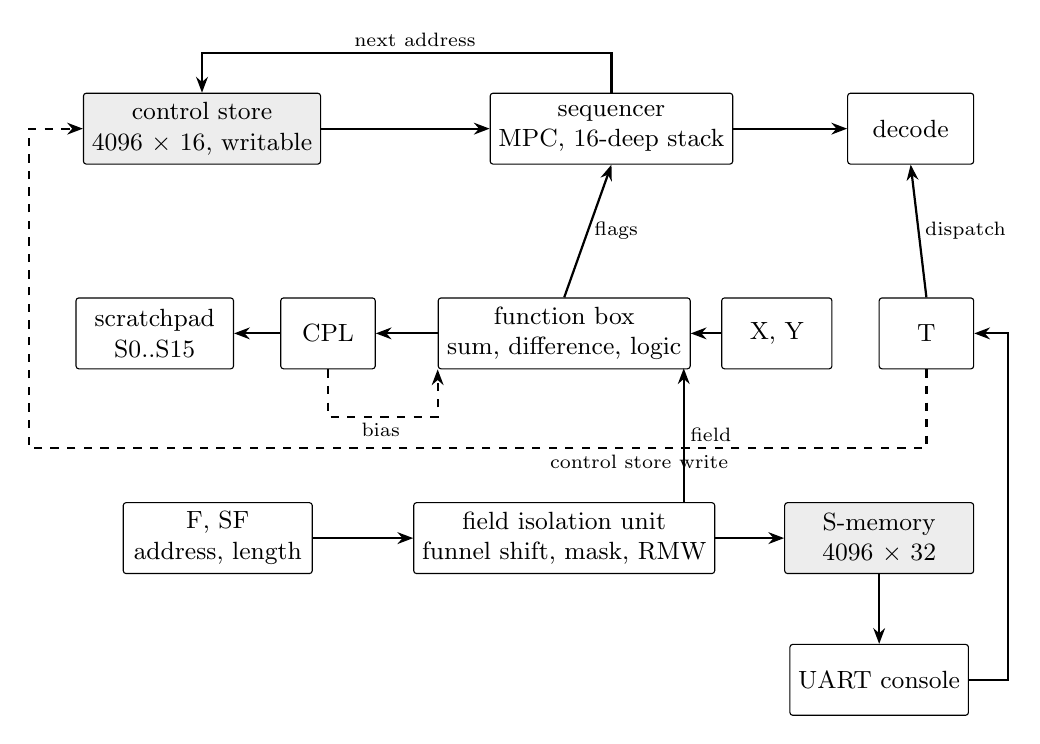
\begin{tikzpicture}[
  font=\small,
  box/.style={draw, rounded corners=1pt, align=center, inner sep=3pt,
              minimum height=9mm},
  mem/.style={box, fill=black!7},
  >={Stealth[length=2mm]},
  ln/.style={->, thick},
  dsh/.style={->, thick, dashed},
  lb/.style={font=\scriptsize, inner sep=2pt},
]

\node[mem, minimum width=30mm] (cs) at (0,0)
     {control store\\ 4096 $\times$ 16, writable};
\node[box, minimum width=30mm] (seq) at (5.2,0)
     {sequencer\\ MPC, 16-deep stack};
\node[box, minimum width=16mm] (dec) at (9.0,0) {decode};

\node[box, minimum width=20mm] (sp) at (-0.6,-2.6) {scratchpad\\ S0..S15};
\node[box, minimum width=12mm] (cpl) at (1.6,-2.6) {CPL};
\node[box, minimum width=32mm] (fn) at (4.6,-2.6)
     {function box\\ sum, difference, logic};
\node[box, minimum width=14mm] (xy) at (7.3,-2.6) {X, Y};
\node[box, minimum width=12mm] (t) at (9.2,-2.6) {T};

\node[box, minimum width=24mm] (desc) at (0.2,-5.2)
     {F, SF\\ address, length};
\node[box, minimum width=34mm] (fiu) at (4.6,-5.2)
     {field isolation unit\\ funnel shift, mask, RMW};
\node[mem, minimum width=24mm] (sm) at (8.6,-5.2)
     {S-memory\\ 4096 $\times$ 32};
\node[box, minimum width=22mm] (uart) at (8.6,-7.0) {UART console};

\draw[ln] (cs.east) -- (seq.west);
\draw[ln] (seq.east) -- (dec.west);
\draw[ln] (seq.north) -- ++(0,5mm) -| node[lb, above, pos=0.24]
      {next address} (cs.north);

\draw[ln] (xy.west) -- (fn.east);
\draw[ln] (fn.west) -- (cpl.east);
\draw[ln] (cpl.west) -- (sp.east);
\draw[dsh] (cpl.south) -- ++(0,-6mm) -| node[lb, below, pos=0.24]
      {bias} (fn.south west);
\draw[ln] (fn.north) -- node[lb, right] {flags} (seq.south);

\draw[ln] (desc.east) -- (fiu.west);
\draw[ln] (fiu.east) -- (sm.west);
\draw[ln] (fiu.north east) ++(-4mm,0) -- node[lb, right] {field}
      ++(0,17mm);
\draw[ln] (sm.south) -- (uart.north);
\draw[ln] (uart.east) -- ++(5mm,0) |- (t.east);

\draw[ln] (t.north) -- node[lb, right] {dispatch} (dec.south);
\draw[dsh] (t.south) -- ++(0,-10mm) -- node[lb, below, pos=0.32]
      {control store write} ++(-11.4,0) |- (cs.west);

\end{tikzpicture}
\caption{The micromachine, with the bias path and the control store
write path drawn dashed.}
\label{fig:arch}
\end{figure}

Memory accesses take three cycles for a read and four for a write, the
cost of synchronous block RAM plus the read-modify-write required for
insertion. Every other microinstruction completes in one cycle: the
address of the next microinstruction is a combinational function of the
one now executing, so taken transfers cost no bubble.

\section{RV32I as an S-language}
\label{sec:rv32i}

The first interpreter implements the full RV32I base integer set in 838
microwords, using six dispatch pages and six shared microsubroutines.
The interpreted machine state occupies a block of S-memory: the
thirty-two architectural registers at bit address $32N$, the program
counter, and interpreter working cells.

Instruction fetch is a single counting read: the field descriptor
supplies the address, the access returns the instruction word, and the
counting mode advances the descriptor by the access length, so the
program counter increments as a side effect of the fetch. Decode is an
extraction of the seven-bit opcode followed by a dispatch, one
microinstruction from field to handler.

One consequence of defined-field addressing deserves to be stated on
its own, because it removes work rather than adding it. Register file
addressing requires no shifter and no multiply. The rs1 field of an
RV32I instruction occupies bits 19 down to 15; extracting ten bits from
position 10 leaves the register number with five junk bits below it,
and masking the result with 0x3E0 yields the register number multiplied
by 32, which is precisely the bit address of that register in S-memory.
Five microinstructions, no hardware. What is normally an address
computation becomes a field extraction.

Misaligned loads and stores are similarly free. A word load from an
address that is not a multiple of four is an ordinary defined-field
read of 32 bits at a bit address that is not a multiple of 32, and the
field isolation unit already spans two memory words for every access.
No microcode branch, no trap, no alignment check.

The interpreter is verified at three levels. Each RTL module is checked
against a golden model in a cocotb suite. The interpreter is compared
instruction by instruction against a Python instruction set simulator
on programs covering arithmetic, logic, shifts, comparisons, all six
branch conditions, loads and stores of every width, and calls through
JAL and JALR. Finally the official riscv-tests rv32ui
suite~\cite{riscvtests} is run in full: 42 tests of 42 pass, including ma\_data, the misaligned data
access test.

The compliance suite earned its place by finding a defect that the
hand-written tests could not. In the shift-right handler the bit
selecting between logical and arithmetic shift was tested after the
source operand had been loaded into the register that produces the zero
flag, so the branch tested the operand rather than the instruction bit.
Logical and arithmetic right shifts agree on non-negative operands, so
every hand-written case passed; only the compliance suite exercised a
negative operand under a logical shift.

\section{Writable control store and the resident loader}
\label{sec:store}

A control store write microinstruction makes the instruction set
mutable at run time. The loader that uses it, named after the B1700
resident interpreter interface, occupies 314 microwords and is written
entirely in microcode. It accepts three binary commands over the serial
line, one to write a block of microwords into the control store, one to
write a block of words into S-memory, and one to jump to microaddress
zero and start whatever interpreter has been loaded.

A halted machine wakes into the loader when the first byte arrives, the
modern reading of the console cassette of the original: a machine at
rest is still addressable from the operator's terminal. Reset enters
the loader at its banner, and the wake path enters past it, so that
binary streams never race the transmitter.

The loader also exports console services at frozen microaddresses, the
arrangement in which interpreters call the resident routine rather than
carry their own input and output. Three services suffice: emit a byte,
print a register as eight hexadecimal digits, and print a
zero-terminated string read from S-memory one byte at a time as a
defined field. The RV32I system-call handler uses them to print the
value of a0 when a program ends. Listing~\ref{lst:console} shows a
session on the board.

\begin{figure}[!htb]
\begin{lstlisting}[caption={A console session on the board, in which
the RV32I interpreter is started and reports its result.},
label={lst:console}]
== B2026 soft machine ==
after the Burroughs B1700: the ISA lives in the store
G: run loaded interpreter   ?: this menu
L/M: binary loader blocks (b26_send.py)
B26> G
a0=00000037
\end{lstlisting}
\end{figure}

\section{Two S-languages on one bitstream}
\label{sec:swap}

The second S-language is a byte-coded stack machine with eight
operations, implemented in 75 microwords. Push and pop are single
counting accesses through the second field descriptor, which is the
read-and-pop and write-and-push of the original expressed directly: the
access returns or stores the datum and the counting mode moves the
stack pointer, in one microinstruction. Its addition handler is five
microinstructions long.

Table~\ref{tab:slang} lists what the same bitstream ran during the
measurements reported below. The third row is the limiting case: six
microwords loaded straight into the control store, no interpreter and
no instruction set at all, which is what it means for the hardware to
define none.

\begin{table}[!htb]
\centering
\caption{Three workloads run on one unchanged bitstream, exchanged over
the serial line.}
\label{tab:slang}
\begin{tabular}{@{}lrrl@{}}
\toprule
Workload & Microwords & Upload (bytes) & Console output \\
\midrule
RV32I interpreter & 838 & 1810 & \texttt{a0=000000D2} \\
Stack machine & 75 & 179 & \texttt{0000000F} \\
Bare microprogram & 6 & 24 & \texttt{0000002A} \\
\bottomrule
\end{tabular}
\end{table}

\section{Results}
\label{sec:results}

All figures in this section are post-place-and-route on a Gowin
GW1NR-LV9QN88PC6/I5 at 27 MHz with no PLL, using Gowin EDA V1.9.12.
Each core is given the same wrapper: one inferred block RAM holding
code and data, one wait state, the same power-on reset, and six active
low LEDs latched by a store to a fixed address. Nothing else is
attached. The workload is the same in every case, a loop summing the
integers from 1 to 100 followed by a store of the low six bits, 305
executed RV32I instructions.

Table~\ref{tab:compare} gives the comparison. Read plainly, the soft
machine loses on every axis that a fixed-ISA core is optimized for: it
costs nine times the logic of SERV, runs at a lower clock, and needs
more cycles per instruction than either SERV or PicoRV32.

\begin{table}[!htb]
\centering
\caption{Four RV32I implementations on the same board, wrapper,
constraint and workload.}
\label{tab:compare}
\begin{tabular}{@{}lrrrrrrl@{}}
\toprule
Core & LUT & ALU & FF & BSRAM & Fmax & CPI & Instruction set \\
\midrule
Glacial & 236 & 38 & 108 & 8 & 66.7 & $\approx$953 & fixed \\
SERV & 283 & 21 & 210 & 9 & 53.9 & 46.6 & fixed \\
PicoRV32 & 1097 & 211 & 446 & 10 & 46.3 & 5.0 & fixed \\
This work & 2569 & 387 & 461 & 12 & 29.7 & 81.3 & writable, swappable \\
\bottomrule
\end{tabular}
\end{table}

Glacial's cycle count is an instruction-mix average rather than a
completed run. Using the core's own instruction-retire trace point, the
reference workload retires 10000 instructions in 9538641 cycles. The
program does not terminate in our harness, the interpreted program
counter returning to zero after the fifth instruction in a manner
consistent with a trap taken while the trap vector is still zero. Since
Glacial passes the compliance suite upstream we attribute this to our
environment, in which the microcode was assembled locally because the
repository ships no prebuilt image, and we therefore report only the
figure the instruction counter measures directly. Every other number in
the table comes from a completed run or from synthesis, and every
synthesis reported zero setup and zero hold violations.

Two details in the table repay attention. Flip-flop counts are close,
461 here against 446 for PicoRV32, while logic cell counts differ by a
factor of two and a half, so the cost of a definable machine sits in
combinational logic rather than in state: the funnel shifter of the
field isolation unit, the mask generator driven by CPL, and a function
box that computes all of its outputs every cycle. And the depth of the
critical path, 5 logic levels for SERV, 6 for PicoRV32 and 15 here, is
the bias mechanism measured in logic levels, the price in nanoseconds
of a machine that reshapes itself every cycle. The path runs from the
CPL register through mask generation, the carry chain, the variable bit
select that produces the length-biased carry, the sequencer condition
multiplexer and the target adder, back to the control store address.

Adding the console and the writable store to the core cost 41 LUT and
70 flip-flops, under one and a half percent of the design, so a machine
that can rewrite its own instruction set and talk to an operator is
nearly free at this scale. The synthesis report records the change in
another way: with a read-only control store the tool inferred four of
the twelve block RAMs as ROM, and once the write port was added all
twelve became read-write.

\section{Discussion}

The comparison table has no column for the property the design pays
for. Three fixed cores implement one instruction set each, chosen when
the bitstream was built. This one implements none, and acquires one
when an interpreter is loaded. During the measurements above the same
configured device was, in sequence, a RISC-V processor, a stack
machine, and a bare microprogram, at a cost of a few hundred bytes and
about a second per change.

Whether that is worth 2300 LUTs depends entirely on what the machine is
for, and the honest answer for most embedded uses is that it is not. A
reader who wants a small RV32I core should use SERV or Glacial. The
cases where a definable machine earns its area are the ones Wilner
identified: an application whose natural machine is not RISC-V, a
teaching setting where the point is that instruction sets are software,
or a system that must change its interpreted language without a
synthesis run.

The measurements also suggest where the design should go next, and the
suggestions come from cycle counts rather than from taste. Assembling
the scattered immediate fields of branch and jump instructions by
repeated doubling costs about fifty microinstructions per taken
transfer; sign extension by exclusive-or and subtract costs six each
time; variable shifts are bit-serial. A signed extraction variant, an
immediate-assembly assist and a barrel shift step are each a handful of
LUTs and would together remove most of the gap to Glacial in cycles
while leaving the architecture unchanged.

A larger question follows from the observation that a lookup table is
itself a memory. If the cost of a definable machine sits in
combinational logic, and combinational logic on an FPGA is already
stored in configuration memory, then a machine whose arithmetic and
control functions are all block RAM lookups would report almost no
logic cells at all, at the price of many cycles and many memory bits.
That is the natural extreme of the same argument and the subject of
ongoing work.

\section{Conclusion}

The B1700 premise can be stated as a measurement, and on a 8640-LUT
FPGA the measurement is this: a machine with no instruction set costs
2569 logic cells and 12 block RAMs, runs RV32I at 81 cycles per
instruction with full rv32ui compliance and free misaligned access, and
exchanges its instruction set over a serial line in about a second.
Fixed-ISA cores on the same board are between two and nine times
smaller and between two and sixteen times faster per instruction. The
trade Wilner described in 1972 is still a trade, and it is now
inexpensive enough to make deliberately.

\section*{Availability}

The design, microcode, verification suites, comparison wrappers and
console tools are available at \url{https://github.com/senolgulgonul/b2026}.

\section*{Acknowledgements}

The comparison would not have been possible without the authors of
SERV, PicoRV32 and Glacial, who publish complete and buildable sources.

\begin{thebibliography}{9}

\bibitem{wilner1972}
W.~T. Wilner,
\emph{B1700 Design and Implementation},
Burroughs Corporation, Santa Barbara Plant, Goleta, California, May 1972.

\bibitem{wilkes1951}
M.~V. Wilkes,
The best way to design an automatic calculating machine,
in \emph{Report of the Manchester University Computer Inaugural
Conference}, Manchester, 1951, pp. 16--18.

\bibitem{barton1970}
R.~S. Barton,
Ideas for computer systems organization: a personal survey,
in \emph{Software Engineering}, vol.~1, Academic Press, New York, 1970,
pp. 7--16.

\bibitem{lonergan1961}
W.~Lonergan and P.~King,
Design of the B5000 system,
\emph{Datamation}, vol.~7, no.~5, May 1961, pp. 28--32.

\bibitem{freeman2004}
M.~Freeman,
A minimal CISC processor architecture for field programmable gate
arrays,
in \emph{Euromicro Conference / DSD Symposium 2004, Work in Progress
Session}, Rennes, France, 2004.

\bibitem{serv}
O.~Kindgren,
SERV: the award-winning bit-serial RISC-V core,
\url{https://github.com/olofk/serv}.

\bibitem{picorv32}
C.~Wolf,
PicoRV32: a size-optimized RISC-V CPU,
\url{https://github.com/YosysHQ/picorv32}.

\bibitem{glacial}
E.~Smith,
Glacial: a microcoded RISC-V core designed for low FPGA resource
utilization,
\url{https://github.com/brouhaha/glacial}.

\bibitem{riscvtests}
RISC-V Software Source,
riscv-tests,
\url{https://github.com/riscv-software-src/riscv-tests}.

\end{thebibliography}

\end{document}
